

\tikzset{every picture/.style={line width=0.75pt}} %set default line width to 0.75pt        

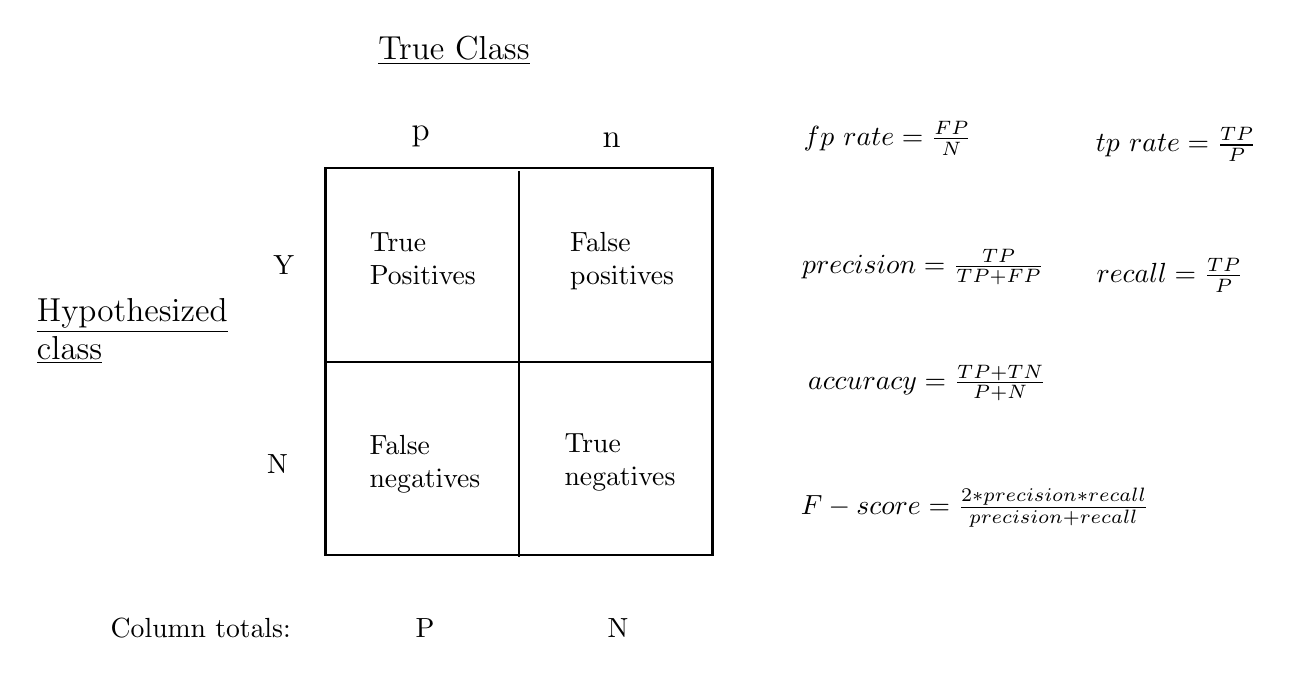
\begin{tikzpicture}[x=0.75pt,y=0.75pt,yscale=-1,xscale=1,thick,scale=1, every node/.style={scale=1}]
%uncomment if require: \path (0,380); %set diagram left start at 0, and has height of 380

%Shape: Square [id:dp7426323050252599] 
\draw   (152.13,94.38) -- (338.5,94.38) -- (338.5,280.75) -- (152.13,280.75) -- cycle ;
%Straight Lines [id:da08397904354123575] 
\draw    (245.31,95.88) -- (245.31,281.92) ;


%Straight Lines [id:da28737204711696407] 
\draw    (152.29,187.56) -- (338.33,187.56) ;





% Text Node
\draw (200,237) node  [align=left] {False\\negatives};
% Text Node
\draw (294,236) node  [align=left] {True\\negatives};
% Text Node
\draw (295,139) node  [align=left] {False\\positives};
% Text Node
\draw (199,138) node  [align=left] {True\\Positives};
% Text Node
\draw (198,79) node  [align=left] {{\large p}};
% Text Node
\draw (290,81) node  [align=left] {{\large n}};
% Text Node
\draw (132,141) node  [align=left] {Y};
% Text Node
\draw (129,237) node  [align=left] {N};
% Text Node
\draw (214,38) node  [align=left] {{\large \underline{True Class}}};
% Text Node
\draw (59,173) node  [align=left] {{\large \underline{Hypothesized}}\\{\large \underline{class}}};
% Text Node
\draw (440,142) node   {$precision=\frac{TP}{TP+FP}$};
% Text Node
\draw (559,146) node   {$recall=\frac{TP}{P}$};
% Text Node
\draw (92,316) node  [align=left] {Column totals:};
% Text Node
\draw (200,316) node  [align=left] {P};
% Text Node
\draw (293,316) node  [align=left] {N};
% Text Node
\draw (423,80) node   {$fp\ rate=\frac{FP}{N}$};
% Text Node
\draw (562,83) node   {$tp\ rate=\frac{TP}{P}$};
% Text Node
\draw (442,198) node   {$accuracy=\frac{TP+TN}{P+N}$};
% Text Node
\draw (465,258) node   {$F-score=\frac{2*precision*recall}{precision+recall}$};


\end{tikzpicture}
